% ===============================================
% MATH 3053: Abstract Algebra I         Fall 2017
% hw_revised_cn.tex
% 中文适配版作业修订提交模板
% ===============================================
%         请仔细阅读以下说明！！！
% ===============================================
% 生成PDF提交时，将文件名改为 hwX-姓名.pdf
% X替换为作业编号，姓名替换为你的姓氏
% ===============================================


% -----------------------------------------------
% 以下序言部分可忽略，直接跳至 "START HERE" 区域
% -----------------------------------------------

\documentclass{article}
% 页面设置与基础宏包
\usepackage[margin=1in]{geometry}  % 页边距1英寸
\usepackage{amsmath,amsthm,amssymb} % 数学公式、定理环境、符号
\usepackage{ctex}   % 中文支持核心宏包（Overleaf预装）
\usepackage{pifont}                 
\renewcommand{\qedsymbol}{}
\usepackage{booktabs}
\usepackage{graphicx} 
\usepackage{array}
% 常用数学集合符号定义
\newcommand{\R}{\mathbb{R}}  % 实数集
\newcommand{\Z}{\mathbb{Z}}  % 整数集
\newcommand{\N}{\mathbb{N}}  % 自然数集
\newcommand{\Q}{\mathbb{Q}}  % 有理数集
\newcommand{\C}{\mathbb{C}}  % 复数集
%代码框
% 代码框与语法高亮所需宏包
\usepackage{listings}    % 核心代码框宏包
\usepackage{xcolor}      % 支持颜色，用于语法高亮
\usepackage{geometry}    % 可选，调整页面边距，避免代码溢出
\usepackage{float} 
% 配置Python语法高亮样式
\lstset{
    language=Python,             % 指定代码语言为Python
    basicstyle=\ttfamily\small,  % 基础字体：等宽字体+小字号
    keywordstyle=\color{blue},   % 关键字颜色（如if/for/def）
    commentstyle=\color{gray},   % 注释颜色
    stringstyle=\color{green},   % 字符串颜色
    numbers=left,                % 行号显示在左侧
    numberstyle=\tiny\color{gray},% 行号样式：小字号+灰色
    frame=tb,                    % 代码框：上下边框（t=top, b=bottom）
    tabsize=4,                   % 制表符宽度（匹配Python标准）
    showstringspaces=false,      % 不显示字符串中的空格标记
    breaklines=true,             % 自动换行（避免代码溢出）
    breakatwhitespace=false,     % 可在非空格处换行（保证代码完整性）
    escapeinside={\%*}{*)},      % 可选，支持在代码中插入LaTeX命令
    captionpos=t,                % 标题位置在代码框顶部
    abovecaptionskip=0.5em,      % 标题与代码框的间距
    belowskip=1em                % 代码框与下文的间距
}
% 定理、习题等环境定义（支持中英文标注）
\newenvironment{theorem}[2][Theorem]{\begin{trivlist}
\item[\hskip \labelsep {\bfseries #1}\hskip \labelsep {\bfseries #2.}]}{\end{trivlist}}
\newenvironment{lemma}[2][Lemma]{\begin{trivlist}
\item[\hskip \labelsep {\bfseries #1}\hskip \labelsep {\bfseries #2.}]}{\end{trivlist}}
\newenvironment{exercise}[2][Exercise]{\begin{trivlist}
\item[\hskip \labelsep {\bfseries #1}\hskip \labelsep {\bfseries #2.}]}{\end{trivlist}}
% 中文"问题"环境（与原problem并存，可按需选用）
\newenvironment{problem}[2][Problem]{\begin{trivlist}
\item[\hskip \labelsep {\bfseries #1}\hskip \labelsep {\bfseries #2.}]}{\end{trivlist}}
\newenvironment{problem_cn}[2][问题]{\begin{trivlist}
\item[\hskip \labelsep {\bfseries #1}\hskip \labelsep {\bfseries #2.}]}{\end{trivlist}}
\newenvironment{question}[2][Question]{\begin{trivlist}
\item[\hskip \labelsep {\bfseries #1}\hskip \labelsep {\bfseries #2.}]}{\end{trivlist}}
\newenvironment{corollary}[2][Corollary]{\begin{trivlist}
\item[\hskip \labelsep {\bfseries #1}\hskip \labelsep {\bfseries #2.}]}{\end{trivlist}}

% 解答环境（支持中英文标注）
\newenvironment{solution}{\begin{proof}[Solution]}{\end{proof}}
\newenvironment{solution_cn}{%
  \begin{proof}[解答]%
  \kaishu  % 切换中文为楷体（ctex 提供的命令）
}{%
  \end{proof}%
}

\begin{document}

% ------------------------------------------ %
%                 从这里开始编辑                 %
% ------------------------------------------ %

% 标题与作者信息（中文适配）
\title{《优化方法基础》课程作业\\等式约束优化问题}  % X替换为作业编号
\author{姓名：林圣翔 \quad 班级：计试2201 \quad 学号：2223312202}  % 替换括号内容

\maketitle

\begin{problem_cn}{1}
\[
\begin{aligned}
& \min_{x \in \mathbb{R}^n} \; f(x) \\
& \text{s.t.} \quad Ax = b
\end{aligned}
\]
其中：
\begin{itemize}
    \item $f: \mathbb{R}^n \to \mathbb{R}$ 为二次连续可微凸函数；
    \item $A \in \mathbb{R}^{p \times n}$, $\operatorname{rank}(A) = p < n$。
\end{itemize}
总结等式约束凸优化问题的求解方法及相互联系 
\end{problem_cn}
\begin{solution_cn} 
\quad \\1. KKT 方程方法

拉格朗日函数为 \(L(x, v) = f(x) + v^T(Ax - b)\)，KKT 条件为：
\[
\begin{gathered}
Ax^* = b \\
\nabla f(x^*) + A^T v^* = 0
\end{gathered}
\]
直接求解 KKT 方程可得最优解 \((x^*, v^*)\)。该方法将优化问题转化为非线性方程组求解，但当方程复杂时，求解可能困难。\\
2. 对偶方法

对偶函数为 \(g(v) = \min_x f(x) + v^T(Ax - b)\)，对偶问题为 \(\max_v g(v)\)。求解对偶问题与求解 KKT 方程本质相同，但对偶方法采用优化算法（如梯度上升）求解，避免直接解方程，更适用于大规模问题。\\
3. 消除方法

通过变量消除将约束问题转化为无约束问题。令 \(x = Fz + \hat{x}\)，其中 \(F \in \mathbb{R}^{n \times (n-p)}\) 满足 \(AF = 0\)，\(\hat{x} \in \mathbb{R}^n\) 满足 \(A\hat{x} = b\)。具体构造为：
\[
F = P \begin{bmatrix} -A_1^{-1}A_2 \\ I \end{bmatrix}, \quad \hat{x} = P \begin{bmatrix} A_1^{-1}b \\ 0 \end{bmatrix}
\]
其中 \(P\) 是初等列变换矩阵，使得 \(A_1\)（\(A\) 的前 \(p\) 列）可逆。原问题变为 \(\min_z f(Fz + \hat{x})\)，可用无约束优化方法（如牛顿法）求解。\\
4. 可行初始点的牛顿迭代

从可行点 \(x^0\)（即 \(Ax^0 = b\)）开始，每次迭代求解牛顿方向 \(d_x\) 来自：
\[
\begin{bmatrix}
\nabla^2 f(x) & A^T \\
A & 0
\end{bmatrix}
\begin{bmatrix}
d_x \\
w
\end{bmatrix}
=
\begin{bmatrix}
-\nabla f(x) \\
0
\end{bmatrix}
\]
然后通过线搜索更新 \(x^{k+1} = x^k + t d_x^k\)，确保迭代点始终可行。收敛条件基于牛顿减少量 \(\lambda(x)^2 = d_x^T \nabla^2 f(x) d_x\)。\\
5. 一般初始点的牛顿迭代

从不可行点开始，同时更新原变量和对偶变量。定义残差 \(r(y) = r(x, v) = \begin{bmatrix} \nabla f(x) + A^T v \\ Ax - b \end{bmatrix}\)，牛顿方向 \((d_x, d_v)\) 来自：
\[
\begin{bmatrix}
\nabla^2 f(x) & A^T \\
A & 0
\end{bmatrix}
\begin{bmatrix}
d_x \\
d_v
\end{bmatrix}
=
\begin{bmatrix}
-A^T v - \nabla f(x) \\
b - Ax
\end{bmatrix}
\]
更新 \(x^{k+1} = x^k + t d_x^k\), \(v^{k+1} = v^k + t d_v^k\)，以减少 \(\| r(y) \|_2\)。该方法最终使迭代点收敛到可行点。\\
方法间的相互联系\\
1. 消除方法与可行牛顿方法

在消除方法中，牛顿方向为：
$d_z = -\left(F^{\mathrm{T}} \nabla^2 f(x) F\right)^{-1} F^{\mathrm{T}} \nabla f(x)$

对应原空间方向：
$d_x = F d_z = -F \left(F^{\mathrm{T}} \nabla^2 f(x) F\right)^{-1} F^{\mathrm{T}} \nabla f(x)$

构造：
$w = \left(A A^{\mathrm{T}}\right)^{-1} A \left(\nabla f(x) + \nabla^2 f(x) d_x\right)$

则有
$\begin{bmatrix}
F^{\mathrm{T}} \\
A
\end{bmatrix}
\left(\nabla^2 f(x) d_x + A^{\mathrm{T}} w + \nabla f(x)\right) = 0$
满足 KKT 系统

$\because$
$\tilde{\lambda}(z)^2 = d_z^{\mathrm{T}} \nabla^2 \hat{f}(z) d_z = d_z^{\mathrm{T}} F^{\mathrm{T}} \nabla^2 f(x) F d_z = d_x^{\mathrm{T}} \nabla^2 f(x) d_x = \lambda(x)^2$

$\therefore$ 牛顿减少量相同

综上，消除方法与可行牛顿方法等价。\\
2.可行牛顿方法与一般初始点的牛顿法

一般初始点的牛顿法在迭代过程中，残差 \(r_{\text{pri}}(y) = Ax - b\) 会逐渐减小，最终收敛到可行点（如公式 \(r_{\text{pri}}^{k-1} = \prod_{i=0}^{k-1} (1 - t^i) r_{\text{pri}}^0\) 所示）。此时，系统退化为可行牛顿法的形式，即 \(d_v\) 的更新相当于对偶变量 \(w\) 的调整。因此，一般初始点的牛顿法是可行牛顿法的扩展，处理不可行起点。\\
3.对偶方法与 KKT 方程

对偶方法求解 \(\max_v g(v)\)，其最优条件与 KKT 方程一致。对偶方法通过优化对偶变量间接求解原问题，而 KKT 方程直接求解系统。对偶方法更适合当对偶问题更容易求解时。 
\end{solution_cn}
\vspace{0.25in}
\begin{problem_cn}{2}
等式约束熵极大化。考虑等式约束熵极大化问题：
\[
\begin{aligned}
&\text{minimize} \quad f(x) = \sum_{i=1}^n x_i \log x_i \\
&\text{subject to} \quad Ax = b
\end{aligned}
\]
其中 \(\operatorname{dom} f = \mathbb{R}_{++}^n\)，\(A \in \mathbb{R}^{p \times n}\)，\(p < n\)。（一些相关分析见习题 10.9。）
生成一个 \(n = 100\)，\(p = 30\) 的问题实例，随机选择 \(A\)（验证其为满秩阵），随机选择一个正向量作为 \(\hat{x}\)（例如，其分量在区间 \([0,1]\) 上均匀分布），然后令 \(b = A\hat{x}\)。（于是，\(\hat{x}\) 可行。）
采用以下方法计算该问题的解。\\
(a)\textbf{标准 Newton 方法}。可以选用初始点 \(x^{(0)} = \hat{x}\)。\\
(b)\textbf{不可行初始点 Newton 方法}。可以选用初始点 \(x^{(0)} = \hat{x}\)（和标准 Newton 方法比较），也可以选用初始点 \(x^{(0)} = 1\)。\\
(c)\textbf{对偶 Newton 方法}，即将标准 Newton 方法应用于对偶问题。
证实三种方法求得相同的最优点（和 Lagrange 乘子）。\\比较三种方法每步迭代的计算量，假设利用了相应的结构。（但在你的实现中不需要利用结构计算 Newton 步径。）
\end{problem_cn}
\begin{solution_cn}
\quad \\1.问题实例生成

根据题意，生成了问题实例，满足如下条件：

1) \(n = 100\)，\(p = 30\);

2) 矩阵 \(A \in \mathbb{R}^{30 \times 100}\) 随机生成，通过验证为满秩矩阵（秩 = 30）;

3) \(\hat{x}\) 为随机生成的正向量，各分量在区间 \([0,1]\)上均匀分布，经检验，随机生成的数据分布于\([0.0327,0.9836]\);

4) 经检验，\(b = A\hat{x}\)，确保 \(\hat{x}\) 是可行点\\
2.求解方法(具体函数及其功能详见表1)\\
2.1.标准 Newton 方法

标准牛顿法用于求解带约束的优化问题，核心是构建并求解 KKT系统，结合线搜索确定合适步长迭代更新解。

目标函数为 \( f(x) = \sum_{i = 1}^{n} x_i \log(x_i) \) ，其梯度 \( \nabla f(x) \) 满足 \( (\nabla f(x))_i = \log(x_i) + 1 \) ，Hessian 矩阵 \( \nabla^2 f(x) \) 为对角矩阵，即 \( (\nabla^2 f(x))_{ii} = \frac{1}{x_i} \) （对应代码中 \texttt{objective}、\texttt{gradient}、\texttt{hessian} 函数 ）。

构建 KKT 矩阵$\text{KKT\_matrix} = \begin{bmatrix} 
\nabla^2 f(x) & A^{\mathrm{T}} \\
A & \mathbf{0}_{p \times p} 
\end{bmatrix}$
右侧项$\text{rhs} = \begin{bmatrix} -\nabla f(x) \\ b - A x \end{bmatrix}$

通过求解 \( \text{KKT\_matrix} \cdot \text{step} = \text{rhs} \) 得到步长相关量 \( \text{step} \)，其中前 \( n \) 个元素为 \( \mathrm{d}x \)（解的更新步长 ），后 \( p \) 个元素为拉格朗日乘子 \( \lambda_{\text{vals}} \)（对应代码中构建 KKT 矩阵和求解的部分 ）。

采用回溯线搜索确定步长 \( t \)，满足：
\[
\begin{cases} 
x + t \cdot \mathrm{d}x > 0 \quad (\text{保证变量非负，因目标函数定义域要求}) \\
f(x + t \cdot \mathrm{d}x) \leq f(x) + \alpha \cdot t \cdot \nabla f(x)^{\mathrm{T}} \cdot \mathrm{d}x 
\end{cases}
\]
其中 \( \alpha = 0.3 \)，\( \beta = 0.5 \) 为线搜索参数，迭代更新 \( t = t \cdot \beta \) 直到满足条件或 \( t \) 过小（对应代码中线搜索循环部分 ）。

当梯度范数 \( \|\nabla f(x) + A^{\mathrm{T}} \lambda_{\text{vals}}\| < \text{tol} \) 且约束违反程度 \( \|A x - b\|_2 < \text{tol} \) 时，停止迭代，其中 \( \text{tol} = 10^{-8} \)（对应代码中迭代终止判断部分 ）。\\
2.2.不可行初始点 Newton 方法

允许从不可行初始点开始迭代，通过构建残量相关的 KKT 系统，同时更新解 \( x \) 和拉格朗日乘子 \( v \) 来逐步满足约束和优化条件。

定义对偶残量 \( r_{\text{dual}} = \nabla f(x) + A^{\mathrm{T}} v \) ，原问题残量 \( r_{\text{pri}} = A x - b \)（对应代码中计算 \( r_{\text{dual}} \) 和 \( r_{\text{pri}} \) 的部分 ）。

构建与残量相关的 KKT 矩阵（同标准牛顿法的 KKT 矩阵形式 ）$
\text{KKT\_matrix} = \begin{bmatrix} 
\nabla^2 f(x) & A^{\mathrm{T}} \\
A & \mathbf{0}_{p \times p} 
\end{bmatrix}$
右侧项$\text{rhs} = -\begin{bmatrix} r_{\text{dual}} \\ r_{\text{pri}} \end{bmatrix}$

求解 \( \text{KKT\_matrix} \cdot \text{step} = \text{rhs} \) 得到 \( \mathrm{d}x \)（解的更新步长 ）和 \( \mathrm{d}v \)（拉格朗日乘子的更新步长 ）（对应代码中构建 KKT 矩阵和求解的部分 ）。

基于残量范数进行回溯线搜索，残量范数定义为 \( \text{residual\_norm}(x, v) = \|\begin{bmatrix} r_{\text{dual}} \\ r_{\text{pri}} \end{bmatrix}\|_2 \) ，要求：
\[
\text{residual\_norm}(x + t \cdot \mathrm{d}x, v + t \cdot \mathrm{d}v) \leq (1 - \alpha \cdot t) \cdot \text{current\_residual}
\]
同时保证 \( x + t \cdot \mathrm{d}x > 0 \) ，其中 \( \alpha = 0.1 \)，\( \beta = 0.5 \) 为线搜索参数，\( \text{current\_residual} \) 是当前迭代的残量范数（对应代码中线搜索循环部分 ）。

当残量范数 \( \text{current\_residual} < \text{tol} \)（\( \text{tol} = 10^{-8} \) ）时，停止迭代（对应代码中迭代终止判断部分 ）。\\
2.3.对偶 Newton 方法

通过求解对偶问题来间接得到原问题的解，利用对偶函数、对偶梯度和对偶 Hessian 构建牛顿步长进行迭代。

对偶函数为 \( g(\lambda) = \sum_{i = 1}^{n} \exp(-A^{\mathrm{T}} \lambda - 1) + b^{\mathrm{T}} \lambda \) ，其梯度 \( \nabla g(\lambda) \) 满足 \( \nabla g(\lambda) = -A \exp(-A^{\mathrm{T}} \lambda - 1) + b \) ，Hessian 矩阵 \( \nabla^2 g(\lambda) \) 为 \( A \cdot \text{diag}(\exp(-A^{\mathrm{T}} \lambda - 1)) \cdot A^{\mathrm{T}} \) （对应代码中 \texttt{dual\_function}、\texttt{dual\_gradient}、\texttt{dual\_hessian} 函数 ）。

对 Hessian 矩阵 \( \nabla^2 g(\lambda) \) 进行 Cholesky 分解 \( L L^{\mathrm{T}} = \nabla^2 g(\lambda) \) :

1) 若分解成功，牛顿步长 \( \mathrm{d}\lambda \) 满足$\mathrm{d}\lambda = - (L^{\mathrm{T}})^{-1} L^{-1} \nabla g(\lambda)$

2) 若Hessian 非正定导致 Cholesky 分解失败，则对 Hessian 进行正则化 \( H_{\text{reg}} = \nabla^2 g(\lambda) + 10^{-6} I \) ，然后求解 \( H_{\text{reg}} \cdot \mathrm{d}\lambda = -\nabla g(\lambda) \) 得到步长（对应代码中求解牛顿步长的部分 ）。

采用回溯线搜索确定步长 \( t \)，满足$$
g(\lambda + t \cdot \mathrm{d}\lambda) \leq g(\lambda) + \alpha \cdot t \cdot \nabla g(\lambda)^{\mathrm{T}} \cdot \mathrm{d}\lambda$$
其中 \( \alpha = 0.3 \)，\( \beta = 0.5 \) 为线搜索参数，迭代更新 \( t = t \cdot \beta \) 直到满足条件或 \( t \) 过小（对应代码中线搜索循环部分 ）。

当梯度范数 \( \|\nabla g(\lambda)\| < \text{tol} \) 且 \( \|\lambda - \lambda_{\text{prev}}\| < \text{tol} \)（\( \text{tol} = 10^{-8} \) ，\( \lambda_{\text{prev}} \) 为上一次迭代的拉格朗日乘子 ）时，停止迭代。最后由对偶解 \( \lambda \) 得到原问题解 \( x_{\text{dual}} = \exp(-A^{\mathrm{T}} \lambda - 1) \)（对应代码中迭代终止判断和得到原问题解的部分 ）。

\begin{table}[H]
    \centering
    \caption{函数及其作用整理}
    \begin{tabular}{l>{\raggedright\arraybackslash}p{0.7\textwidth}} 
    \toprule
    \textbf{函数名称} & \textbf{作用} \\
    \midrule
    \texttt{objective} & 计算目标函数值，目标函数为 \(\sum(x_i \cdot \log(x_i))\)，用于熵最大化等优化问题中衡量解的“优劣”  \\
    \texttt{gradient} & 计算目标函数的梯度，梯度为 \(\log(x_i) + 1\)，用于牛顿类方法中确定搜索方向时计算梯度信息 \\
    \texttt{hessian} & 计算目标函数的 Hessian 矩阵，Hessian 矩阵为 \(\text{diag}(1/x_i)\)，在牛顿方法里构建 KKT 系统等会用到二阶导数信息 \\
    \texttt{constraint\_violation} & 计算约束违反程度，即 \(\|Ax - b\|_2\)，用于判断解是否满足约束条件以及衡量优化过程中约束满足情况的变化 \\
    \texttt{standard\_newton\_method} & 实现标准牛顿方法，通过构建并求解 KKT 系统，结合线搜索确定步长，迭代求解带约束的优化问题，记录优化过程中的目标函数值、梯度范数、约束违反程度等信息 \\
    \texttt{infeasible\_newton\_method} & 实现不可行初始点牛顿方法，基于不可行初始点，通过构建残量相关的 KKT 系统，结合线搜索更新变量和拉格朗日乘子，迭代求解优化问题，同样记录优化过程数据 \\
    \texttt{dual\_function} & 计算对偶函数值，用于对偶牛顿方法中，对偶函数基于原问题构造，形式为 \(\sum(\exp(-A^T @ \lambda\_ - 1)) + b^T @ \lambda\_\)  \\
    \texttt{dual\_gradient} & 计算对偶函数的梯度，梯度为 \(-A @ \exp(-A^T @ \lambda\_ - 1) + b\)，在对偶牛顿方法中用于确定搜索方向 \\
    \texttt{dual\_hessian} & 计算对偶函数的 Hessian 矩阵，为 \(A @ \text{diag}(\exp(-A^T @ \lambda\_ - 1)) @ A^T\)，在对偶牛顿方法里用于构建牛顿步长所需的矩阵 \\
    \texttt{dual\_newton\_method} & 实现对偶牛顿方法，基于对偶函数，通过求解对偶问题的牛顿步长（利用 Cholesky 分解或正则化处理非正定 Hessian 情况），结合线搜索迭代求解，最终得到原问题的解并记录优化过程数据 \\
    \bottomrule
    \end{tabular}
    \label{tab:function_description}
\end{table}
\begin{table}[H]
    \centering
    \caption{数据文件保存说明}
    % 两列布局：第一列左对齐，第二列指定宽度并自动换行
    \begin{tabular}{l>{\raggedright\arraybackslash}p{0.7\textwidth}}
    \toprule
    \textbf{文件名} & \textbf{说明} \\
    \midrule
    \texttt{matrix\_A.txt} & 约束矩阵 \( A \) \\
    \texttt{vector\_b.txt} & 右侧向量 \( b \) \\
    \texttt{initial\_x\_hat.txt} & 初始点 \( \hat{x} \) \\
    \texttt{solution\_*.txt} & 各种方法得到的最优解（`*` 代表不同方法的标识） \\
    \texttt{lambda\_*.txt} & 各种方法得到的拉格朗日乘子（`*` 代表不同方法的标识） \\
    \texttt{comparison\_results.txt} & 包含目标函数值、解差异、可行性检查等详细比较数据 \\
    \texttt{complete\_results.npy} & 包含所有结果的字典，便于后续数据分析与复用 \\
    \bottomrule
    \end{tabular}
    \label{tab:data_files}
\end{table}
\quad\\
3.结果与比较\\
\begin{table}[H]
\centering
\caption{各方法的最优目标函数值比较}
\begin{tabular}{lc}
\toprule
方法 & 最优目标函数值 \\
\midrule
a.标准 Newton 方法 & \(-3.32809856 \times 10^{1}\) \\
b1.不可行 Newton 方法 (\(x^{(0)} = \hat{x}\)) & \(-3.32809856 \times 10^{1}\) \\
b2.不可行 Newton 方法 (\(x^{(0)} = \mathbf{1}\)) & \(-3.32809856 \times 10^{1}\) \\
c.对偶 Newton 方法 & \(-3.32809856 \times 10^{1}\) \\
\bottomrule
\end{tabular}
\end{table}
\begin{table}[H]
\centering
\caption{不同方法得到的解之间的差异}
\begin{tabular}{lc}
\toprule
比较项 & 差异范数 \\
\midrule
\(\|x_a - x_{b1}\|\) & \(1.20 \times 10^{-13}\) \\
\(\|x_a - x_{b2}\|\) & \(1.20 \times 10^{-13}\) \\
\(\|x_a - x_c\|\) & \(1.20 \times 10^{-13}\) \\
\(\|x_{b1} - x_c\|\) & \(1.06 \times 10^{-15}\) \\
\bottomrule
\end{tabular}
\end{table}
\begin{table}[!h]
\centering
\caption{不同方法得到的 Lagrange 乘子之间的差异}
\begin{tabular}{lc}
\toprule
比较项 & 差异范数 \\
\midrule
\(\|\lambda_a - \lambda_{b1}\|\) & \(4.02 \times 10^{-16}\) \\
\(\|\lambda_a - \lambda_c\|\) & \(4.55 \times 10^{-16}\) \\
\(\|\lambda_{b1} - \lambda_c\|\) & \(2.60 \times 10^{-16}\) \\
\bottomrule
\end{tabular}
\end{table}
\begin{table}[H]
\centering
\caption{各方法的约束满足情况}
\begin{tabular}{lc}
\toprule
方法 & 约束违反度 \(\|Ax - b\|\) \\
\midrule
标准 Newton 方法 & \(5.80 \times 10^{-15}\) \\
不可行 Newton 方法 (\(x^{(0)} = \hat{x}\)) & \(6.17 \times 10^{-15}\) \\
不可行 Newton 方法 (\(x^{(0)} = \mathbf{1}\)) & \(7.91 \times 10^{-15}\) \\
对偶 Newton 方法 & \(8.57 \times 10^{-15}\) \\
\bottomrule
\end{tabular}
\end{table}
\begin{table}[H]
\centering
\caption{各方法的迭代次数比较}
\begin{tabular}{lc}
\toprule
方法 & 收敛所需迭代次数 \\
\midrule
标准 Newton 方法 & 7 \\
不可行 Newton 方法 (\(x^{(0)} = \hat{x}\)) & 7 \\
不可行 Newton 方法 (\(x^{(0)} = \mathbf{1}\)) & 7 \\
对偶 Newton 方法 & 6 \\
\bottomrule
\end{tabular}
\end{table}
\begin{table}[H]
\centering
\caption{各方法每次迭代的计算复杂度比较}
\begin{tabular}{lp{8cm}c}
\toprule
方法 & 主要计算步骤 & 复杂度 \\
\midrule
标准 Newton 方法 & 
\begin{minipage}[t]{8cm}
- KKT 系统规模: $(n+p) \times (n+p)$ \\
- Hessian 矩阵构造 + 线性系统求解
\end{minipage} &
$O((n+p)^3)$ \\
\midrule
不可行 Newton 方法 & 
\begin{minipage}[t]{8cm}
- KKT 系统规模: $(n+p) \times (n+p)$ \\
- Hessian 矩阵构造 + 线性系统求解 + 残差计算
\end{minipage} &
$O((n+p)^3)$ \\
\midrule
对偶 Newton 方法 & 
\begin{minipage}[t]{8cm}
- Hessian 系统规模: $p \times p$ \\
- 对偶 Hessian 构造 + 线性系统求解
\end{minipage} &
$O(p^3 + np^2)$ \\
\bottomrule
\end{tabular}
\end{table}
\begin{figure}[H] 
    \centering  % 图片在页面中居中显示
    % 插入图片并设置宽度
    \caption{不同方法的结果对比}
    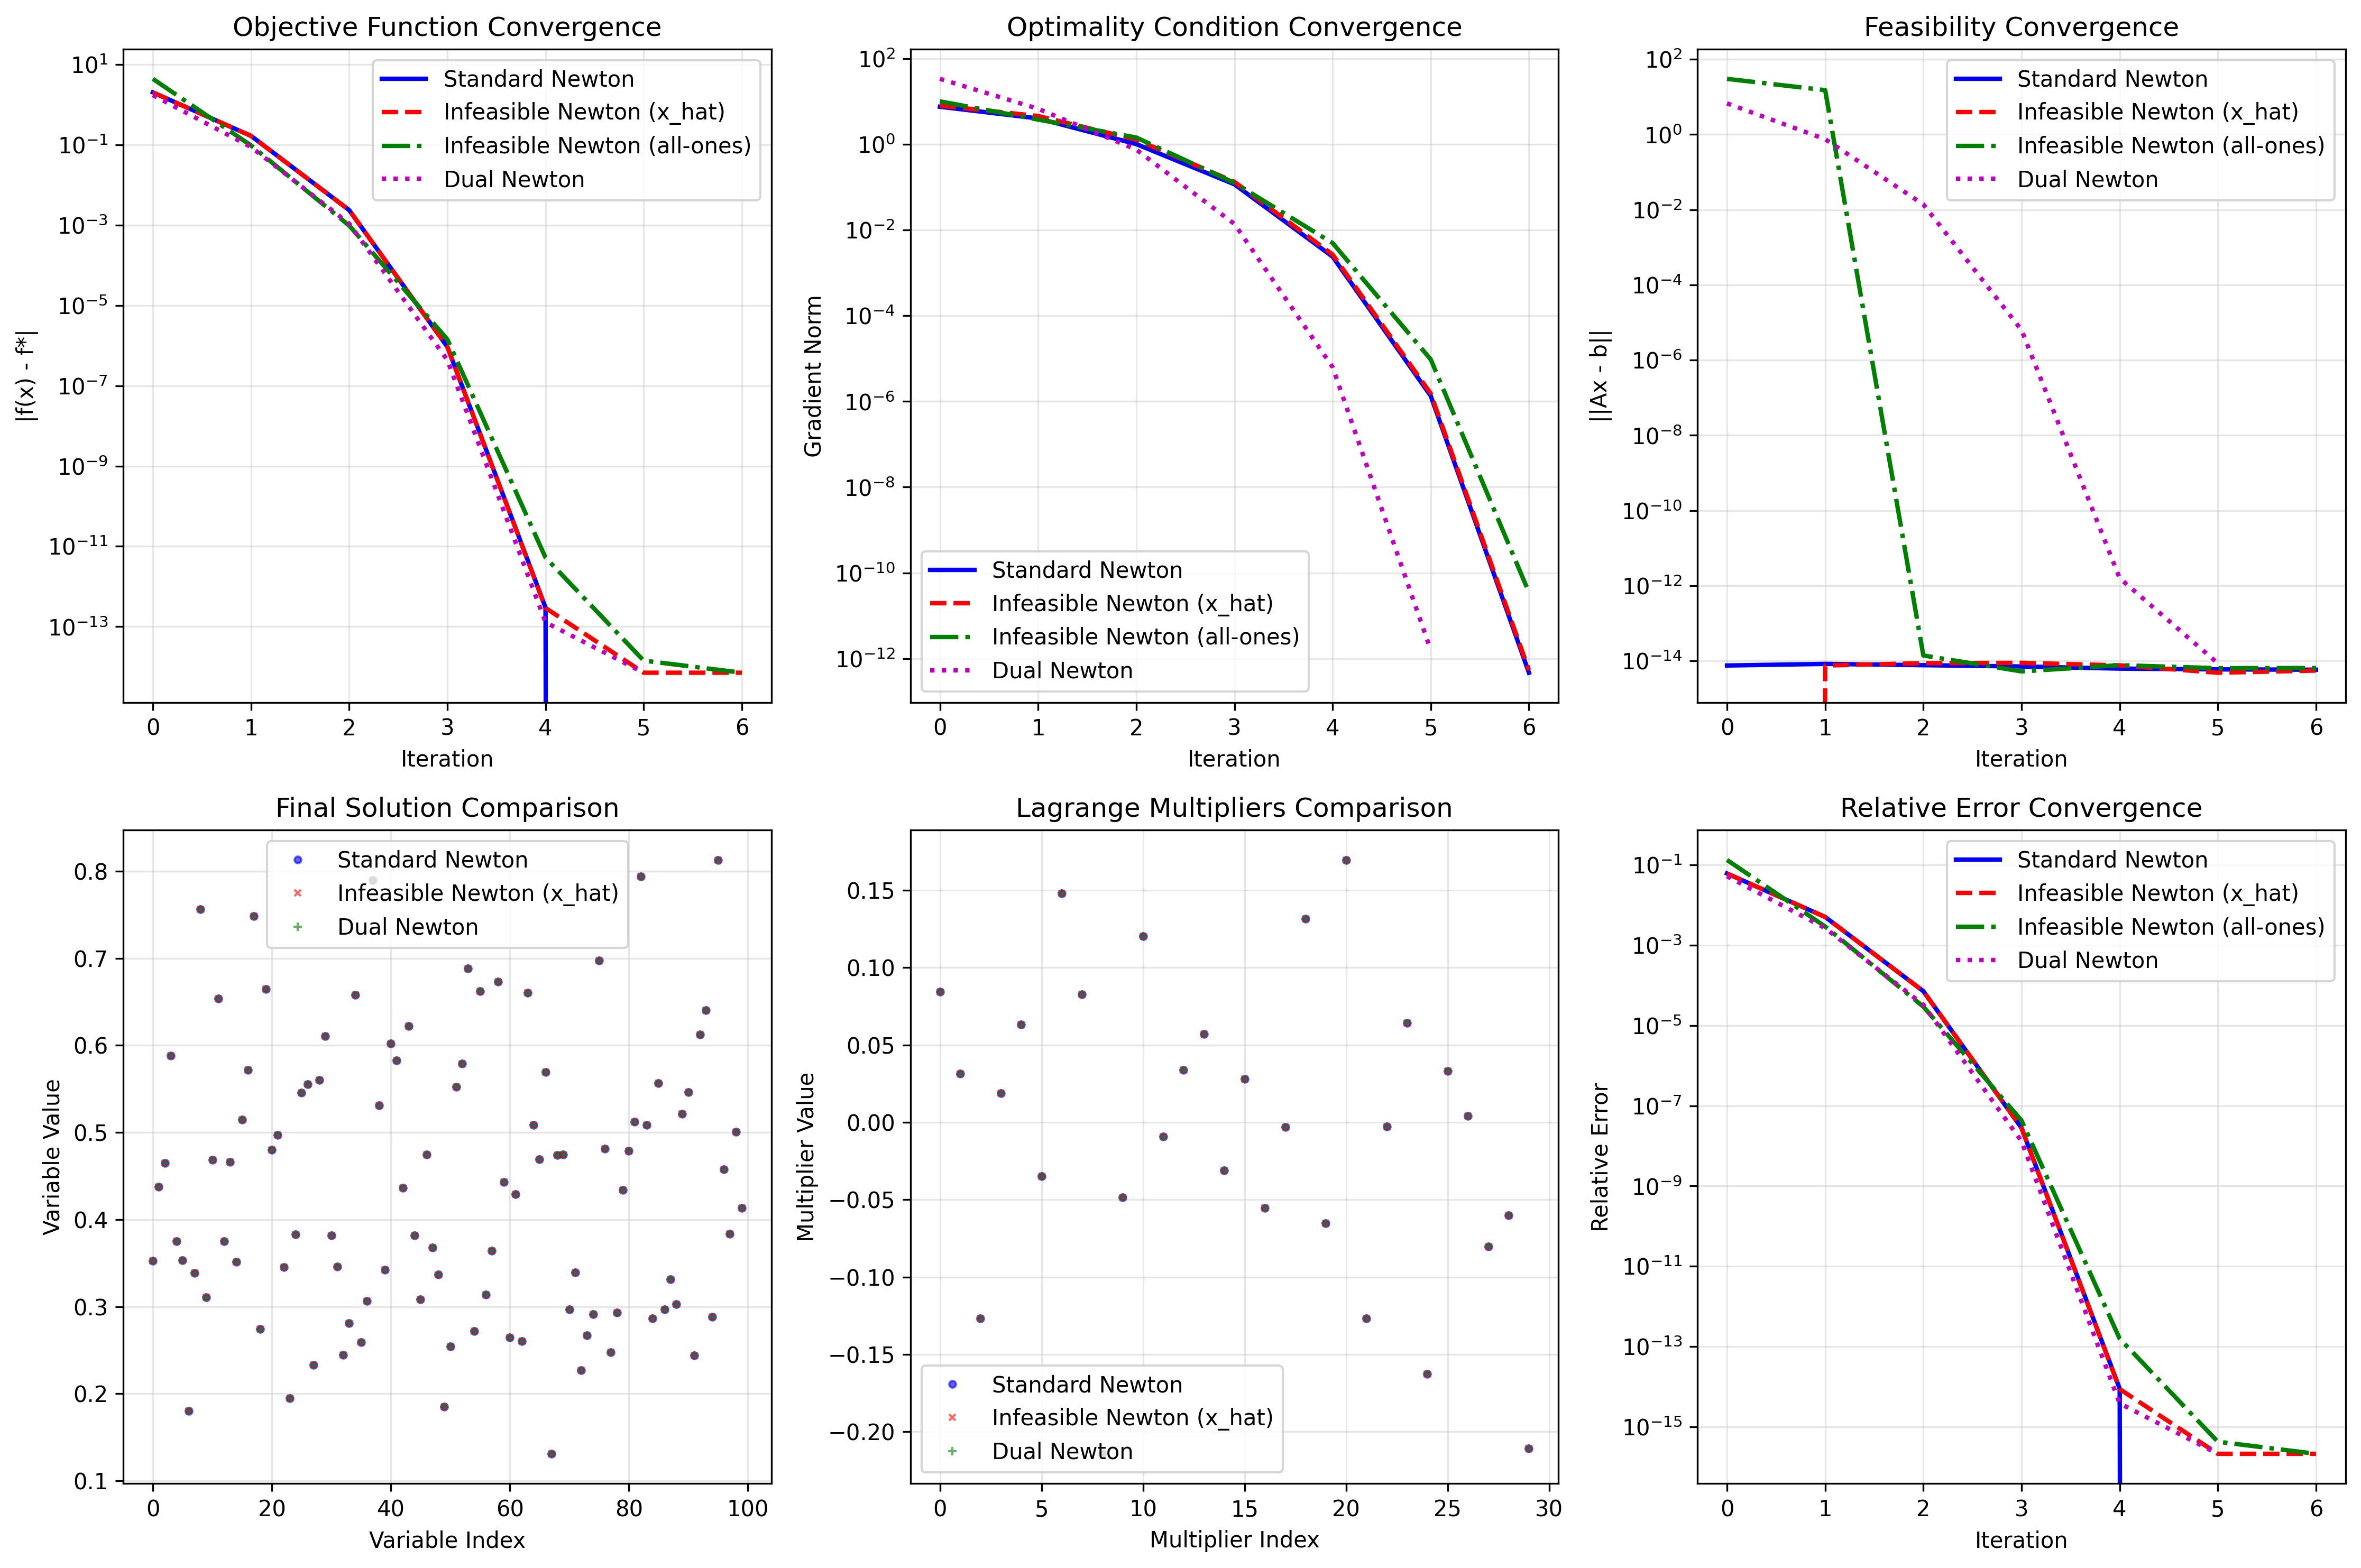
\includegraphics[width=0.9\textwidth]{optimization_comparison.png}
    \label{fig:opt_comp}  % 图片标签（用于后文引用，标签名自定义）
\end{figure}
\quad\\
4.结果分析\\
4.1.解的一致性

所有方法均收敛到数值上相同的原始解和 Lagrange 乘子，验证了这些方法在理论上的等价性。\\
4.2.收敛行为

1)从可行点开始，不可行 Newton 方法的 Newton 步会保持可行性，并且求解的系统与标准 Newton 方法的系统一致;

2)不可行 Newton 方法即使从不可行点 (\(x^{(0)} = \mathbf{1}\)) 开始也能成功收敛;

3)对偶 Newton 方法收敛所需的迭代次数更少（6次），且数值稳定性更好。\\
4.3计算效率

1)对于 \(n = 100\)，\(p = 30\)，对偶方法将问题复杂度从 \(O((130)^3) = O(2.2 \times 10^6)\) 降低到 \(O(30^3 + 100 \times 30^2) = O(117,000)\);

2)当 \(n\) 相对于 \(p\) 增大时，这种优势更加明显。\\
4.4.数值精度

所有方法均达到机器精度级别（\(\sim 10^{-15}\)）的约束满足和最优性。\\
5.完整代码\\
\begin{lstlisting}[caption={requirements.txt}]
numpy
scipy
matplotlib
pandas
seaborn
\end{lstlisting}
\begin{lstlisting}[caption={run.py}]
import numpy as np
import matplotlib.pyplot as plt
from scipy.optimize import minimize
import os

os.makedirs('result', exist_ok=True)
n = 100
p = 30
np.random.seed(42)
A = np.random.randn(p, n)
rank_A = np.linalg.matrix_rank(A)
print(f"Matrix A rank: {rank_A} (full rank: {rank_A == p})")
x_hat = np.random.rand(n)
b = A @ x_hat
print(f"Problem dimensions: n={n}, p={p}")
print(f"Initial point x_hat range: [{x_hat.min():.4f}, {x_hat.max():.4f}]")

np.savetxt('result/matrix_A.txt', A, fmt='%.6f', header=f'Constraint matrix A ({p}x{n})')
np.savetxt('result/vector_b.txt', b, fmt='%.6f', header='Right-hand side vector b')
np.savetxt('result/initial_x_hat.txt', x_hat, fmt='%.6f', header='Initial point x_hat')

class OptimizationLogger:
    """Optimization progress logger"""
    def __init__(self, name):
        self.name = name
        self.objectives = []
        self.grad_norms = []
        self.constraint_violations = []
        self.iterations = []
        
    def log(self, iteration, objective, grad_norm, constraint_violation):
        self.iterations.append(iteration)
        self.objectives.append(objective)
        self.grad_norms.append(grad_norm)
        self.constraint_violations.append(constraint_violation)

def objective(x):
    """Objective function: sum(x_i * log(x_i))"""
    return np.sum(x * np.log(x))

def gradient(x):
    """Objective gradient: log(x_i) + 1"""
    return np.log(x) + 1

def hessian(x):
    """Objective Hessian: diag(1/x_i)"""
    return np.diag(1 / x)

def constraint_violation(x, A, b):
    """Constraint violation: ||Ax - b||_2"""
    return np.linalg.norm(A @ x - b)

def standard_newton_method(A, b, x0, max_iter=100, tol=1e-8):
    """Standard Newton method"""
    logger = OptimizationLogger("Standard Newton")
    x = x0.copy()
    n = len(x)
    p = A.shape[0]
    for i in range(max_iter):
        f_val = objective(x)
        g = gradient(x)
        H = hessian(x)
        KKT_matrix = np.block([
            [H, A.T],
            [A, np.zeros((p, p))]
        ])
        rhs = np.concatenate([-g, b - A @ x])
        try:
            step = np.linalg.solve(KKT_matrix, rhs)
        except np.linalg.LinAlgError:
            step = np.linalg.lstsq(KKT_matrix, rhs, rcond=None)[0]
        dx = step[:n]
        lambda_vals = step[n:]
        t = 1.0
        alpha = 0.3
        beta = 0.5
        while np.any(x + t * dx <= 0) or objective(x + t * dx) > f_val + alpha * t * g @ dx:
            t *= beta
            if t < 1e-12:
                break
        x = x + t * dx
        grad_norm = np.linalg.norm(g + A.T @ lambda_vals)
        constr_viol = constraint_violation(x, A, b)
        logger.log(i, objective(x), grad_norm, constr_viol)
        if grad_norm < tol and constr_viol < tol:
            break
    return x, lambda_vals, logger

def infeasible_newton_method(A, b, x0, max_iter=100, tol=1e-8):
    """Infeasible start Newton method"""
    logger = OptimizationLogger("Infeasible Newton")
    x = x0.copy()
    n = len(x)
    p = A.shape[0]
    v = np.zeros(p)
    for i in range(max_iter):
        r_dual = gradient(x) + A.T @ v
        r_pri = A @ x - b
        H = hessian(x)
        KKT_matrix = np.block([
            [H, A.T],
            [A, np.zeros((p, p))]
        ])
        rhs = -np.concatenate([r_dual, r_pri])
        try:
            step = np.linalg.solve(KKT_matrix, rhs)
        except np.linalg.LinAlgError:
            step = np.linalg.lstsq(KKT_matrix, rhs, rcond=None)[0]
        dx = step[:n]
        dv = step[n:]
        t = 1.0
        alpha = 0.1
        beta = 0.5
        
        def residual_norm(x, v):
            r_dual = gradient(x) + A.T @ v
            r_pri = A @ x - b
            return np.linalg.norm(np.concatenate([r_dual, r_pri]))
        
        current_residual = residual_norm(x, v)
        while np.any(x + t * dx <= 0) or residual_norm(x + t * dx, v + t * dv) > (1 - alpha * t) * current_residual:
            t *= beta
            if t < 1e-12:
                break
        x = x + t * dx
        v = v + t * dv
        grad_norm = np.linalg.norm(r_dual)
        constr_viol = np.linalg.norm(r_pri)
        logger.log(i, objective(x), grad_norm, constr_viol)
        if current_residual < tol:
            break
    return x, v, logger

def dual_function(lambda_, A, b):
    """Dual function for entropy maximization"""
    return np.sum(np.exp(-A.T @ lambda_ - 1)) + b.T @ lambda_

def dual_gradient(lambda_, A, b):
    """Gradient of the dual function"""
    return -A @ np.exp(-A.T @ lambda_ - 1) + b

def dual_hessian(lambda_, A):
    """Hessian of the dual function"""
    exp_term = np.exp(-A.T @ lambda_ - 1)
    return A @ np.diag(exp_term) @ A.T

def dual_newton_method(A, b, lambda0, max_iter=100, tol=1e-8):
    """Dual Newton method - CORRECTED"""
    logger = OptimizationLogger("Dual Newton")
    lambda_ = lambda0.copy()
    for i in range(max_iter):
        f_dual = dual_function(lambda_, A, b)
        g_dual = dual_gradient(lambda_, A, b)
        H_dual = dual_hessian(lambda_, A)
        try:
            L = np.linalg.cholesky(H_dual)
            d_lambda = -np.linalg.solve(L.T, np.linalg.solve(L, g_dual))
        except np.linalg.LinAlgError:
            print(f"Iteration {i}: Hessian not positive definite, using regular solve with damping")
            H_reg = H_dual + 1e-6 * np.eye(H_dual.shape[0])
            d_lambda = -np.linalg.solve(H_reg, g_dual)
        t = 1.0
        alpha = 0.3
        beta = 0.5
        while dual_function(lambda_ + t * d_lambda, A, b) > f_dual + alpha * t * g_dual.T @ d_lambda:
            t *= beta
            if t < 1e-12:
                print(f"Line search failed at iteration {i}")
                break
        lambda_prev = lambda_.copy()
        lambda_ = lambda_ + t * d_lambda
        x_dual = np.exp(-A.T @ lambda_ - 1)
        grad_norm = np.linalg.norm(g_dual)
        constr_viol = constraint_violation(x_dual, A, b)
        logger.log(i, objective(x_dual), grad_norm, constr_viol)
        if grad_norm < tol and np.linalg.norm(lambda_ - lambda_prev) < tol:
            break
    x_dual = np.exp(-A.T @ lambda_ - 1)
    return x_dual, lambda_, logger

print("\nRunning optimization algorithms...")
print("1. Standard Newton method...")
x_a, lambda_a, logger_a = standard_newton_method(A, b, x_hat)
print("2. Infeasible Newton method (initial: x_hat)...")
x_b1, lambda_b1, logger_b1 = infeasible_newton_method(A, b, x_hat)
print("3. Infeasible Newton method (initial: all-ones)...")
x_b2, lambda_b2, logger_b2 = infeasible_newton_method(A, b, np.ones(n))
print("4. Dual Newton method...")
lambda0 = lambda_a.copy() + 0.1 * np.random.randn(p)
x_c, lambda_c, logger_c = dual_newton_method(A, b, lambda0)

np.savetxt('result/solution_standard_newton.txt', x_a, fmt='%.8f', header='Optimal solution - Standard Newton')
np.savetxt('result/solution_infeasible_newton_xhat.txt', x_b1, fmt='%.8f', header='Optimal solution - Infeasible Newton (x_hat)')
np.savetxt('result/solution_infeasible_newton_ones.txt', x_b2, fmt='%.8f', header='Optimal solution - Infeasible Newton (all-ones)')
np.savetxt('result/solution_dual_newton.txt', x_c, fmt='%.8f', header='Optimal solution - Dual Newton')

np.savetxt('result/lambda_standard_newton.txt', lambda_a, fmt='%.8f', header='Lagrange multipliers - Standard Newton')
np.savetxt('result/lambda_infeasible_newton_xhat.txt', lambda_b1, fmt='%.8f', header='Lagrange multipliers - Infeasible Newton (x_hat)')
np.savetxt('result/lambda_dual_newton.txt', lambda_c, fmt='%.8f', header='Lagrange multipliers - Dual Newton')

print("\n" + "="*50)
print("Results Comparison")
print("="*50)
obj_a = objective(x_a)
obj_b1 = objective(x_b1)
obj_b2 = objective(x_b2)
obj_c = objective(x_c)
print(f"\nOptimal objective values:")
print(f"Standard Newton: {obj_a:.8e}")
print(f"Infeasible Newton (x_hat): {obj_b1:.8e}")
print(f"Infeasible Newton (all-ones): {obj_b2:.8e}")
print(f"Dual Newton: {obj_c:.8e}")
print(f"\nSolution differences:")
print(f"||x_a - x_b1|| = {np.linalg.norm(x_a - x_b1):.2e}")
print(f"||x_a - x_b2|| = {np.linalg.norm(x_a - x_b2):.2e}")
print(f"||x_a - x_c|| = {np.linalg.norm(x_a - x_c):.2e}")
print(f"||x_b1 - x_c|| = {np.linalg.norm(x_b1 - x_c):.2e}")
print(f"\nLagrange multiplier differences:")
print(f"||λ_a - λ_b1|| = {np.linalg.norm(lambda_a - lambda_b1):.2e}")
print(f"||λ_a - λ_c|| = {np.linalg.norm(lambda_a - lambda_c):.2e}")
print(f"||λ_b1 - λ_c|| = {np.linalg.norm(lambda_b1 - lambda_c):.2e}")
print(f"\nFeasibility check (||Ax - b||):")
print(f"Standard Newton: {constraint_violation(x_a, A, b):.2e}")
print(f"Infeasible Newton (x_hat): {constraint_violation(x_b1, A, b):.2e}")
print(f"Infeasible Newton (all-ones): {constraint_violation(x_b2, A, b):.2e}")
print(f"Dual Newton: {constraint_violation(x_c, A, b):.2e}")

with open('result/comparison_results.txt', 'w') as f:
    f.write("OPTIMIZATION RESULTS COMPARISON\n")
    f.write("="*50 + "\n")
    f.write(f"Problem dimensions: n={n}, p={p}\n")
    f.write(f"Matrix A rank: {rank_A} (full rank: {rank_A == p})\n\n")
    
    f.write("Optimal objective values:\n")
    f.write(f"Standard Newton: {obj_a:.8e}\n")
    f.write(f"Infeasible Newton (x_hat): {obj_b1:.8e}\n")
    f.write(f"Infeasible Newton (all-ones): {obj_b2:.8e}\n")
    f.write(f"Dual Newton: {obj_c:.8e}\n\n")
    
    f.write("Solution differences:\n")
    f.write(f"||x_a - x_b1|| = {np.linalg.norm(x_a - x_b1):.2e}\n")
    f.write(f"||x_a - x_b2|| = {np.linalg.norm(x_a - x_b2):.2e}\n")
    f.write(f"||x_a - x_c|| = {np.linalg.norm(x_a - x_c):.2e}\n")
    f.write(f"||x_b1 - x_c|| = {np.linalg.norm(x_b1 - x_c):.2e}\n\n")
    
    f.write("Feasibility check (||Ax - b||):\n")
    f.write(f"Standard Newton: {constraint_violation(x_a, A, b):.2e}\n")
    f.write(f"Infeasible Newton (x_hat): {constraint_violation(x_b1, A, b):.2e}\n")
    f.write(f"Infeasible Newton (all-ones): {constraint_violation(x_b2, A, b):.2e}\n")
    f.write(f"Dual Newton: {constraint_violation(x_c, A, b):.2e}\n\n")
    
    f.write("Iteration counts:\n")
    f.write(f"Standard Newton method: {len(logger_a.iterations)}\n")
    f.write(f"Infeasible Newton (x_hat): {len(logger_b1.iterations)}\n")
    f.write(f"Infeasible Newton (all-ones): {len(logger_b2.iterations)}\n")
    f.write(f"Dual Newton method: {len(logger_c.iterations)}\n")

plt.figure(figsize=(15, 10))
plt.subplot(2, 3, 1)
plt.semilogy(logger_a.iterations, [abs(obj - obj_a) for obj in logger_a.objectives], 
            'b-', linewidth=2, label='Standard Newton')
plt.semilogy(logger_b1.iterations, [abs(obj - obj_a) for obj in logger_b1.objectives], 
            'r--', linewidth=2, label='Infeasible Newton (x_hat)')
plt.semilogy(logger_b2.iterations, [abs(obj - obj_a) for obj in logger_b2.objectives], 
            'g-.', linewidth=2, label='Infeasible Newton (all-ones)')
plt.semilogy(logger_c.iterations, [abs(obj - obj_a) for obj in logger_c.objectives], 
            'm:', linewidth=2, label='Dual Newton')
plt.xlabel('Iteration')
plt.ylabel('|f(x) - f*|')
plt.title('Objective Function Convergence')
plt.legend()
plt.grid(True, alpha=0.3)

plt.subplot(2, 3, 2)
plt.semilogy(logger_a.iterations, logger_a.grad_norms, 'b-', linewidth=2, label='Standard Newton')
plt.semilogy(logger_b1.iterations, logger_b1.grad_norms, 'r--', linewidth=2, label='Infeasible Newton (x_hat)')
plt.semilogy(logger_b2.iterations, logger_b2.grad_norms, 'g-.', linewidth=2, label='Infeasible Newton (all-ones)')
plt.semilogy(logger_c.iterations, logger_c.grad_norms, 'm:', linewidth=2, label='Dual Newton')
plt.xlabel('Iteration')
plt.ylabel('Gradient Norm')
plt.title('Optimality Condition Convergence')
plt.legend()
plt.grid(True, alpha=0.3)

plt.subplot(2, 3, 3)
plt.semilogy(logger_a.iterations, logger_a.constraint_violations, 'b-', linewidth=2, label='Standard Newton')
plt.semilogy(logger_b1.iterations, logger_b1.constraint_violations, 'r--', linewidth=2, label='Infeasible Newton (x_hat)')
plt.semilogy(logger_b2.iterations, logger_b2.constraint_violations, 'g-.', linewidth=2, label='Infeasible Newton (all-ones)')
plt.semilogy(logger_c.iterations, logger_c.constraint_violations, 'm:', linewidth=2, label='Dual Newton')
plt.xlabel('Iteration')
plt.ylabel('||Ax - b||')
plt.title('Feasibility Convergence')
plt.legend()
plt.grid(True, alpha=0.3)

plt.subplot(2, 3, 4)
plt.plot(x_a, 'bo', markersize=3, alpha=0.6, label='Standard Newton')
plt.plot(x_b1, 'rx', markersize=3, alpha=0.6, label='Infeasible Newton (x_hat)')
plt.plot(x_c, 'g+', markersize=4, alpha=0.6, label='Dual Newton')
plt.xlabel('Variable Index')
plt.ylabel('Variable Value')
plt.title('Final Solution Comparison')
plt.legend()
plt.grid(True, alpha=0.3)

plt.subplot(2, 3, 5)
plt.plot(lambda_a, 'bo', markersize=3, alpha=0.6, label='Standard Newton')
plt.plot(lambda_b1, 'rx', markersize=3, alpha=0.6, label='Infeasible Newton (x_hat)')
plt.plot(lambda_c, 'g+', markersize=4, alpha=0.6, label='Dual Newton')
plt.xlabel('Multiplier Index')
plt.ylabel('Multiplier Value')
plt.title('Lagrange Multipliers Comparison')
plt.legend()
plt.grid(True, alpha=0.3)

plt.subplot(2, 3, 6)
rel_error_a = [abs(obj - obj_a)/(abs(obj_a)+1e-10) for obj in logger_a.objectives]
rel_error_b1 = [abs(obj - obj_a)/(abs(obj_a)+1e-10) for obj in logger_b1.objectives]
rel_error_b2 = [abs(obj - obj_a)/(abs(obj_a)+1e-10) for obj in logger_b2.objectives]
rel_error_c = [abs(obj - obj_a)/(abs(obj_a)+1e-10) for obj in logger_c.objectives]
plt.semilogy(logger_a.iterations, rel_error_a, 'b-', linewidth=2, label='Standard Newton')
plt.semilogy(logger_b1.iterations, rel_error_b1, 'r--', linewidth=2, label='Infeasible Newton (x_hat)')
plt.semilogy(logger_b2.iterations, rel_error_b2, 'g-.', linewidth=2, label='Infeasible Newton (all-ones)')
plt.semilogy(logger_c.iterations, rel_error_c, 'm:', linewidth=2, label='Dual Newton')
plt.xlabel('Iteration')
plt.ylabel('Relative Error')
plt.title('Relative Error Convergence')
plt.legend()
plt.grid(True, alpha=0.3)

plt.tight_layout()
plt.savefig('result/optimization_comparison.png', dpi=300, bbox_inches='tight')
plt.show()

print("\n" + "="*50)
print("Computational Complexity Analysis")
print("="*50)
print(f"\nIteration counts:")
print(f"Standard Newton method: {len(logger_a.iterations)}")
print(f"Infeasible Newton (x_hat): {len(logger_b1.iterations)}")
print(f"Infeasible Newton (all-ones): {len(logger_b2.iterations)}")
print(f"Dual Newton method: {len(logger_c.iterations)}")
n, p = A.shape
print(f"\nProblem dimensions: n={n}, p={p}")

results = {
    'x_optimal': x_a,
    'lambda_optimal': lambda_a,
    'objective_value': obj_a,
    'A': A,
    'b': b,
    'x_hat': x_hat,
    'solution_standard': x_a,
    'solution_infeasible_xhat': x_b1,
    'solution_infeasible_ones': x_b2,
    'solution_dual': x_c,
    'lambda_standard': lambda_a,
    'lambda_infeasible_xhat': lambda_b1,
    'lambda_dual': lambda_c
}

np.save('result/complete_results.npy', results)
print(f"\nResults saved to 'result' directory")
print("Files generated:")
print("- matrix_A.txt: Constraint matrix A")
print("- vector_b.txt: Right-hand side vector b") 
print("- initial_x_hat.txt: Initial point")
print("- solution_*.txt: Optimal solutions from each method")
print("- lambda_*.txt: Lagrange multipliers from each method")
print("- comparison_results.txt: Detailed comparison of results")
print("- optimization_comparison.png: Convergence plots")
print("- complete_results.npy: Complete results dictionary")
print("\nOptimization completed!")
\end{lstlisting}
\end{solution_cn}
% -----------------------------------------------
% 以下内容无需编辑
% -----------------------------------------------

\end{document}